% IEEE conference paper root
% Build with pdflatex, not xelatex
% See README for engine rationale
\documentclass[conference]{IEEEtran}

% cite.sty, never biblatex
\usepackage{cite}
\usepackage{amsmath,amssymb,amsfonts}
\usepackage{graphicx}
\usepackage{textcomp}
\usepackage{url}
\usepackage{booktabs}
% Ragged right table columns
\usepackage{array}

% Break long reference URLs
\Urlmuskip=0mu plus 1mu\relax
\makeatletter
\g@addto@macro\UrlBreaks{\do\-}
\makeatother

% Center multi-line figure captions
\makeatletter
\long\def\@makecaption#1#2{%
\ifx\@captype\@IEEEtablestring%
\footnotesize\bgroup\par\centering\@IEEEtabletopskipstrut{\normalfont\footnotesize #1}\\{\normalfont\footnotesize\scshape #2}\par\addvspace{0.5\baselineskip}\egroup%
\@IEEEtablecaptionsepspace
\else
\@IEEEfigurecaptionsepspace
\setbox\@tempboxa\hbox{\normalfont\footnotesize {#1.}\nobreakspace\nobreakspace #2}%
\ifdim \wd\@tempboxa >\hsize%
\parbox[t]{\hsize}{\normalfont\footnotesize\centering {#1.}\nobreakspace\nobreakspace #2\par}%
\else%
\hbox to\hsize{\normalfont\footnotesize\hfil\box\@tempboxa\hfil}%
\fi\fi}
\makeatother

\begin{document}

\title{Development of an Integrated DataOps and MLOps\\Platform Architecture on Kubernetes\\Using Open Source Tools}

\author{\IEEEauthorblockN{1\textsuperscript{st} Bryan P. Hutagalung}
\IEEEauthorblockA{\textit{Information Systems and Technology} \\
\textit{School of Electrical Engineering and Informatics} \\
\textit{Institut Teknologi Bandung} \\
Bandung, Indonesia \\
18222130@std.stei.itb.ac.id}
\and
\IEEEauthorblockN{2\textsuperscript{nd} Achmad Imam Kistijantoro}
\IEEEauthorblockA{\textit{Informatics} \\
\textit{School of Electrical Engineering and Informatics} \\
\textit{Institut Teknologi Bandung} \\
Bandung, Indonesia \\
imam@staff.stei.itb.ac.id}}

\maketitle
% Page numbers, bottom center
\thispagestyle{plain}
\pagestyle{plain}

% Abstract and index terms

\begin{abstract}
DataOps and MLOps are commonly adopted side by side, yet the tools supporting them remain fragmented and the two disciplines are usually run by separate teams. A team that wants both must either assemble the integration itself, which takes time, or subscribe to managed services, which carries recurring cost and ties the platform to one provider. This paper develops an integrated DataOps and MLOps platform architecture on Kubernetes built from open source tools. Design Science Research Methodology guides the work from problem identification through design, GitOps-based implementation, and evaluation. The architecture comprises nine platform layers derived from the convergence of five sources that used different methods rather than from majority adoption, and components for each layer are selected through scored comparison against four criteria. The design joins the two disciplines at three points, namely a shared feature contract, an open lineage protocol feeding one metadata catalog, and one declarative control plane reconciled from a single Git repository. A crypto asset market use case verifies the platform on a single-node cluster. Evaluation covers 26 requirements, of which two are verified functionally, five are instrumented with their targets left unmeasured, and 19 are verified structurally. The retraining chain fires when injected drift crosses the configured threshold, yielding a Population Stability Index of 18.107 against a threshold of 0.2. A cost comparison across three provisioning options places the open source design below fully managed services over three years under an assumed labour allocation. Load characterisation under real traffic remains open, on one node and across a cluster.
\end{abstract}

\begin{IEEEkeywords}
DataOps, drift detection, feature store, GitOps, Kubernetes, MLOps, open source
\end{IEEEkeywords}

% Problem, pressures, contribution

\section{Introduction}
\label{sec:introduction}

DataOps improves the quality and speed of the data flow, while MLOps improves the reliability of the model lifecycle. Teams generally need both. In practice the two grow apart, because the model code is only a small part of a production machine learning system and most of the surrounding work is data management, configuration, monitoring, and serving \cite{sculley2015hidden}. When the two disciplines are operated separately, lineage, drift detection, and feature serving end up inconsistent across the cycle.

Building the combined platform in-house runs into the breadth of the choice space. A systematic mapping of 43 primary studies identifies 35 recurring MLOps architecture components \cite{najafabadi2024analysis}, and open source components in this space tend to stand alone rather than form a cohesive framework \cite{burgueno2025toward}. Integration work, learning curve, and version alignment therefore fall on the adopting team from the start.

The alternative is to subscribe to managed services, which reduces configuration work but introduces recurring cost that is hard to estimate in advance and can become uneconomical as load grows \cite{hamza2024serverlesscost}. Organisations are left choosing between a long build and a subscription with limited room for customisation.

Neither choice removes the integration work between the ingestion, feature, training, and serving layers. Integration is then reassembled per project, and metadata, identity, and lineage are managed separately, so provenance is hard to trace and feature values can differ between training and serving. Surveys of deployment practice report pipeline maintenance and inter-component integration as recurring difficulties \cite{paleyes2022challenges}.

This paper develops an integrated DataOps and MLOps platform architecture on Kubernetes built from open source tools. The architecture combines four properties that prior work has addressed separately, namely DataOps and MLOps unified on one Kubernetes control plane, data governance enforced automatically along the production pipeline, drift detection that triggers retraining through that same declarative control, and a dual-store feature service under one contract with vector search alongside it on a separate index. No individual element is new. The contribution is the combination, which the designs reviewed in Section~\ref{sec:related_work} do not cover together.

% Positioning against four prior works

\section{Related Work}
\label{sec:related_work}

MLOps is defined as a combination of working culture and software that automates experimentation, training, evaluation, deployment, and monitoring \cite{kreuzberger2023mlops}. That definition frames what an integrated platform has to cover on the model side, and DataOps adds ingestion, quality, and governance on the data side \cite{munappy2020adhoc}.

Four studies sit close to this work. Burgue\~{n}o-Romero et al. propose an open source MLOps architecture assembled from components, but a feature service with vector support is not among them \cite{burgueno2025toward}. Amou Najafabadi et al. map MLOps architectures across 43 primary studies, but the mapping does not extend to DataOps \cite{najafabadi2024analysis}. Drift detection and model updating are the emphasis of Rodrigues et al., whose architecture targets near real-time distributed stream learning, though data governance is not enforced as a control plane there \cite{rodrigues2025architecture}. Ahmad et al. discuss MLOps-enabled security strategies without linking them to a governance control plane that enforces access policy across the data and model lifecycle \cite{ahmad2024mlops}.

Because those four properties are handled separately, feature lineage from ingestion through to model serving cannot be traced on one control plane.

A second gap is more specific. Amou Najafabadi et al. observe that an explicit mapping between concrete tools and architecture components is still missing from the MLOps literature \cite{najafabadi2024analysis}. Section~\ref{sec:architecture} supplies that mapping for the open source case, with the scoring shown.

% DSRM phases and objectives

\section{Method}
\label{sec:method}

The work follows Design Science Research Methodology \cite{peffers2007dsrm}. The main output is a running platform, which is an instantiation artifact in the design science taxonomy \cite{hevner2004design}, so an artifact-oriented framework fits better than a pure software engineering process. CRISP-DM and TDSP were considered and set aside, because both organise the building of one model on one data domain, whereas the output here is a cross-domain platform on which a model is only one of the workloads served.

The six phases run iteratively. Problem identification produces four problem statements from a study of DataOps, MLOps, and data governance. Objective definition turns each statement into an artifact that can be installed, operated, and audited, giving four objectives mapped one to one onto the problem statements.

\begin{itemize}
\item \textbf{T-1} unifies ingestion, processing, storage, feature store, training, serving, governance, and observability into one declarative control plane with GitOps practice.
\item \textbf{T-2} builds a data governance sub-system providing metadata catalog, lineage recording, and quality control as shared services along the pipeline.
\item \textbf{T-3} implements automated drift detection with a threshold-based retraining policy, and enforces point-in-time correctness across batch and streaming modes through the historical feature join.
\item \textbf{T-4} develops a dual-store feature service delivering tabular and aggregate features under one API contract, with vector embeddings served on a separate index whose embedding space stays consistent between training and inference.
\end{itemize}

The objectives are decomposed into 14 functional and 12 non-functional requirements, which become the units of evaluation in Section~\ref{sec:evaluation}. Design and development classify the services named by the sources in Section~\ref{subsec:layers} into platform layers, select open source components per layer, and express the result as a declarative control plane. Before that, four provisioning alternatives were scored against the same 26 requirements from vendor documentation and public offerings, and open source on self-managed Kubernetes scored highest, mainly on temporal validity, vector support, portability, and extensibility. That scoring is desk research preceding implementation and is not an evaluation result. It is also separate from the three-way cost comparison in Section~\ref{subsec:cost}, which prices only the options that remained practical. Demonstration installs the platform on k3s and drives it with one real domain use case. Evaluation examines functional fulfilment, non-functional targets, and governance, and communication produces this paper alongside the source repository.

% Layer derivation, selection, bridges, sub-systems

\section{Architecture}
\label{sec:architecture}

% Nine layers, evidence, selected components

\begin{table*}[!t]
\caption{Platform Layers, Their Evidence Base, and the Components Selected for Each}
\label{tab:layer_mapping}
\centering
\footnotesize
\begin{tabular}{@{}>{\raggedright\arraybackslash}p{3.0cm}>{\raggedright\arraybackslash}p{5.4cm}>{\raggedright\arraybackslash}p{1.5cm}>{\raggedright\arraybackslash}p{5.6cm}@{}}
\toprule
\textbf{Layer} & \textbf{Recurring services named by the sources} & \textbf{Sources} & \textbf{Selected open source components} \\
\midrule
Orchestration and Infrastructure & model training infrastructure, infrastructure and supporting services & \cite{kreuzberger2023mlops}, \cite{najafabadi2024analysis}, \cite{googlecloud2024mlops} & k3s, Horizontal Pod Autoscaler, Vertical Pod Autoscaler recommender, KEDA, Kueue, cert-manager \\
Data Ingestion and Processing & data collection, data cleaning, data preprocessor, data ingestion & \cite{amershi2019software}, \cite{najafabadi2024analysis}, \cite{munappy2020adhoc} & Kafka with Strimzi, Karapace, Debezium, Flink, Spark, dbt, Airflow, Trino \\
Data Storage & dataset repository, data storage, data versioning & \cite{najafabadi2024analysis}, \cite{munappy2020adhoc} & MinIO, Apache Iceberg, Lakekeeper, lakeFS, ClickHouse, PostgreSQL, MySQL, OpenSearch \\
Feature Service & feature store, offline and online serving & \cite{kreuzberger2023mlops}, \cite{googlecloud2024mlops}, \cite{najafabadi2024analysis} & Feast, ClickHouse offline, Valkey online, Qdrant on a separate index outside the Feast contract \\
Model Lifecycle & model training, model evaluation, model registry, ML metadata store, inference service & \cite{kreuzberger2023mlops}, \cite{amershi2019software}, \cite{googlecloud2024mlops}, \cite{najafabadi2024analysis} & Kubeflow Pipelines, Katib, Kubeflow Trainer, MLflow, KServe, Knative, Argo Workflows \\
Data Governance & data testing, controlled access, privacy and data integrity protection & \cite{munappy2020adhoc} & DataHub, OpenLineage, Great Expectations \\
Observability & monitoring component, model monitoring, data monitoring & \cite{kreuzberger2023mlops}, \cite{amershi2019software}, \cite{najafabadi2024analysis}, \cite{munappy2020adhoc} & Prometheus, Loki, Grafana Tempo, Grafana, OpenTelemetry, Superset, Evidently, OpenCost \\
GitOps and Continuous Delivery & CI/CD component, source code repository, deployment services & \cite{kreuzberger2023mlops}, \cite{googlecloud2024mlops}, \cite{najafabadi2024analysis} & Argo CD, Gitea, Tekton, Argo Rollouts \\
Security & controlled access, privacy and data security compliance, API gateway & \cite{munappy2020adhoc}, \cite{najafabadi2024analysis} & Istio, APISIX, dex, oauth2-proxy, SpiceDB, OpenBao, Kyverno, Falco \\
\bottomrule
\end{tabular}
\end{table*}


\subsection{Deriving the Platform Layers}
\label{subsec:layers}

The layers are derived from convergence across sources that used different methods, not from majority adoption. On the model side, Kreuzberger et al. name nine MLOps components through mixed-method research combining literature review, tool review, and expert interviews \cite{kreuzberger2023mlops}. Amershi et al. arrive at a nine-stage workflow by observing engineering teams at Microsoft, and already separate the data-oriented stages from the model-oriented ones \cite{amershi2019software}. Starting from different methods, the two name largely the same components. Amou Najafabadi et al. synthesise 35 components from 43 primary studies and report how often each occurs, with model registry at 21 occurrences, ML metadata repository at 15, and feature store at 8 \cite{najafabadi2024analysis}. Google Cloud lists seven components required for MLOps level 2 \cite{googlecloud2024mlops}.

The occurrence counts carry less weight than they suggest, because no single component reaches an absolute majority of the 43 studies. What they show is that the same components recur across independent studies.

On the data side, Munappy et al. derive an evolution model from ad-hoc analytics to DataOps from an industrial case study, naming data collection, data testing, and data monitoring as recurring practices, and treating controlled access and data-integrity protection as governance \cite{munappy2020adhoc}. The data field therefore widens the MLOps set rather than duplicating it. It is the convergence across these five sources of differing method that forms the evidence base, not a claim that any one component is used by most of the industry.

Consolidating both sides gives the nine layers in Table~\ref{tab:layer_mapping}. Four cover the data domain and five cover the model domain and platform operations. Each row traces to the sources that name its services, and the backing is not even across rows. The Model Lifecycle layer is named by four sources at once, whereas the Security layer draws mainly on the security governance dimension of the DataOps side. Table~\ref{tab:layer_mapping} leaves that difference visible instead of levelling it.

Two boundaries are deliberate. Monitoring is placed in Observability rather than in Serving, so that measurement does not mix with inference. Drift detection is not a tenth layer. It is a mechanism that crosses layers, connecting the monitoring function to the model lifecycle, and it is realised as a sub-system instead.

The layer order follows the concept order of the underlying literature study one to one, so the partitioning is not a new taxonomy standing on its own.

\subsection{Selecting Components}
\label{subsec:selection}

Every role with more than one viable candidate is scored in a comparison matrix. Each matrix scores four criteria chosen for that role, so the set is not fixed across matrices. Maturity, community size, and Kubernetes integration recur most often, while the rest are role-specific, such as batch and streaming capability for processing engines or footprint for Kubernetes distributions. Each criterion scores 0, 1, or 2, giving a maximum total of 8. A score of 0 marks a criterion that is not met, 1 marks partial support that still needs an additional component or carries a significant limitation, and 2 marks full support by built-in capability. Scores are derived from official documentation and each project's maintenance status. Twenty-four matrices cover the roles across the nine layers, and their winners appear in the last column of Table~\ref{tab:layer_mapping} alongside the components adopted without a contest. Nineteen of the 24 winners take a perfect 8.

The highest total takes the role, but it does not remove the other candidates. A tool with a lower total can still be adopted where it is stronger on the criterion that matters. Spark takes the highest total and the large-scale batch role, while Flink, which scores lower overall but higher on event-time processing with exactly-once checkpointing, takes the streaming role. Neither displaces the other. Kubeflow Pipelines takes the training flow, Argo Workflows runs the scheduled control loop, and Airflow orchestrates the batch data pipeline. The three roles do not overlap.

\begin{figure*}[!t]
\centering
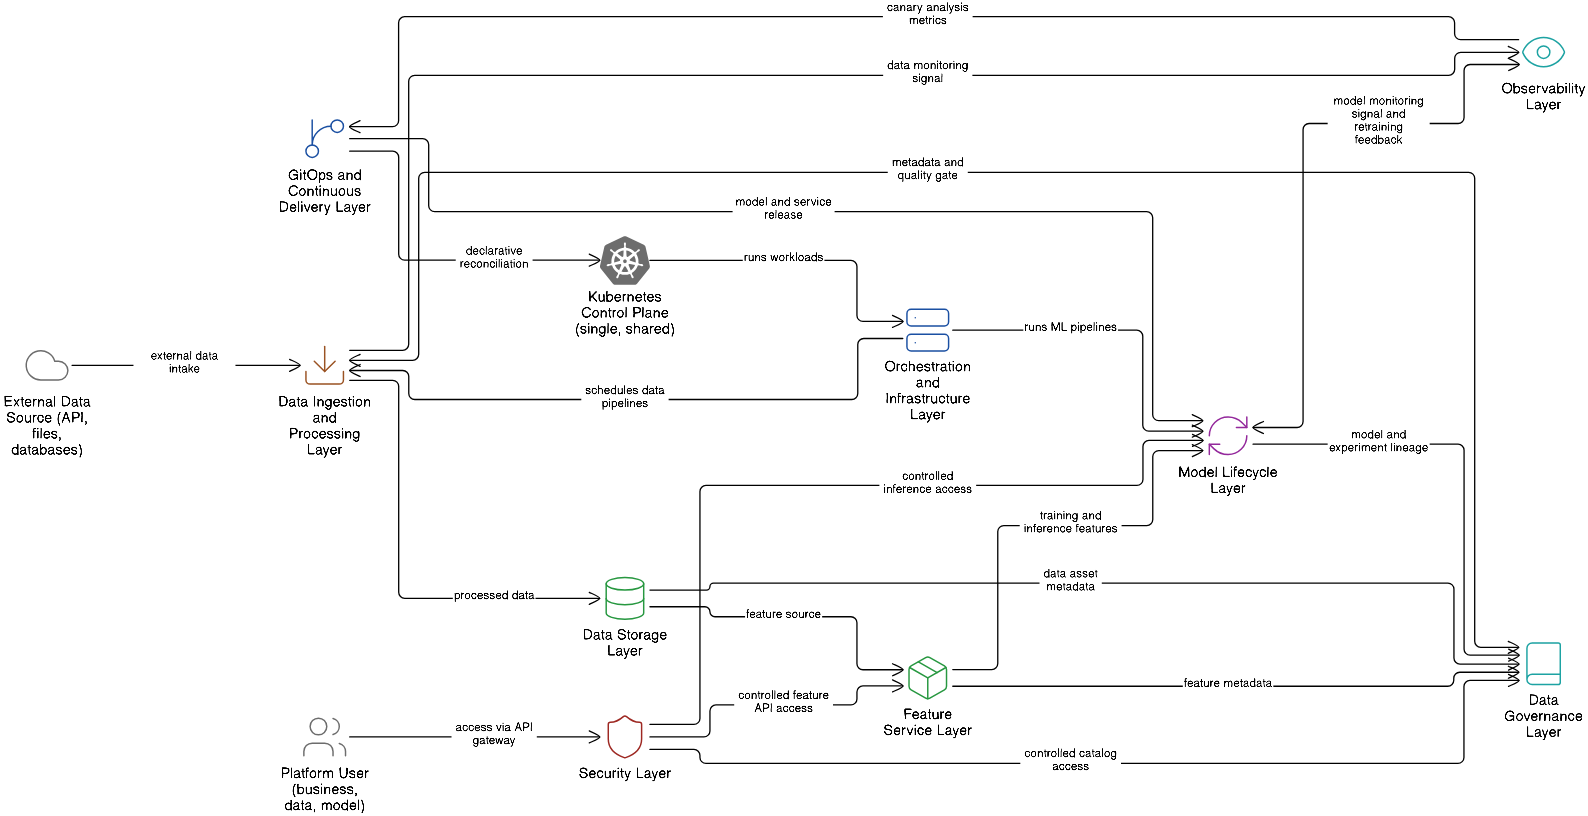
\includegraphics[width=\textwidth]{figures/DataOps_MLOps_Flow.png}
\caption{Integrated service architecture on a shared Kubernetes control plane, drawn without binding to any tool \cite{googlecloud2024mlops}}
\label{fig:architecture}
\end{figure*}

\subsection{Joining the Two Disciplines}
\label{subsec:bridges}

Fig.~\ref{fig:architecture} shows the nine layers as one architecture. DataOps and MLOps meet at three points, and at each one the producing and the consuming side read the same definition rather than two copies of it.

The first is the feature contract. Feast binds the offline store and the online store to one feature definition, so the pipelines that write features and the training and inference code that read them use the same contract.

The second is open lineage. OpenLineage carries transformation events from both the data orchestrator and the training orchestrator, including the SQL transformation steps inside them, into one metadata catalog. The lineage of a training dataset is then traceable from the same graph that holds the ingestion assets.

The third is the declarative control plane. Argo CD reconciles the manifests of both disciplines from one Git repository, so policy and component versions stay consistent across the two. It is also what makes the drift loop of Section~\ref{subsec:drift} declarative.

\subsection{Drift Detection and Retraining}
\label{subsec:drift}

Drift detection sits where the two disciplines meet, because drift is observed on the data layer while its consequence is executed on the model layer. A detector runs as a scheduled job, every 15 minutes for volatile features and hourly for more stable ones. It reads a current window and a reference window from ClickHouse and computes the Population Stability Index with adaptive binning and the Kolmogorov-Smirnov statistic with per-feature thresholds \cite{reis2016kdd}. Scores are written back to an analytics table in ClickHouse for audit, and pushed to Prometheus for alerting.

A scheduled Argo CronWorkflow reads those scores and decides whether to trigger training. Thresholds live in a Git-committed ConfigMap, and each run records a checksum of the configuration version, so a policy change is auditable without inspecting the cluster. When a threshold is crossed, the workflow calls the training pipeline, which assembles its training set through a point-in-time join and logs the run to the model registry as a new version.

Whether that candidate replaces the running model is decided at canary promotion on live serving metrics, not by a separate comparison before deployment. Promotion is configured to halt and roll back when a metric crosses its threshold.

\subsection{Dual-Store Feature Service}
\label{subsec:feature}

The dual-store design is two stores under one contract. ClickHouse holds offline features for training, Valkey serves online lookups at inference, and both derive their schema from the same Feast definition. Vector embeddings are handled separately. Qdrant stands outside Feast as a vector index reached through its native client, because an approximate nearest neighbour load needs memory for the HNSW graph \cite{malkov2020efficient} and behaves differently from a key-value point lookup. Separating them lets each be tuned on its own.

Point-in-time correctness is enforced through the historical feature join, which admits only values whose event timestamp does not exceed each entity row's reference timestamp and still falls inside the feature view's time-to-live. Training therefore sees the values that would have been available at that instant, which is what prevents the optimistic evaluation that leakage produces \cite{kaufman2012leakage}. Batch and stream pipelines write to stores registered on the same feature view, so a consumer does not need to know which pipeline produced a value.

% Environment, GitOps pattern, use case

\section{Implementation}
\label{sec:implementation}

The platform runs on k3s on a single node \cite{kubernetes2024}. The node count is an implementation choice, and moving to a multi-node cluster should change only the Kustomize overlay, a move not yet performed. Library versions and base images are pinned to the highest stable release as of April 2026 so that testing is reproducible, and a component is intended to be replaceable by an equivalent without changing the design.

Components are grouped one namespace per layer and joined by stable API contracts, which lets network policy default to deny with declared exceptions. Argo CD is the only path by which change reaches the cluster \cite{limoncelli2022gitops}, with every component rendered from an ApplicationSet template so adding a component adds no boilerplate. Tekton builds and tests. Istio enforces mutual TLS in strict mode on internal traffic, Kyverno validates at admission, and Falco watches the kernel at runtime. The default is one idle replica per workload, with autoscaling templates prepared but not exercised under load.

Platform code stays domain-agnostic in its own directory, while the domain lives in a separate use-case directory applied through a Kustomize overlay setting only the name prefix, registry mapping, initial replicas, and autoscaling bounds.

The verification use case is crypto asset market analytics on Coinbase data, chosen for three reasons. It exercises all nine layers at once. Crypto markets trade continuously with no closing hours \cite{makarov2020trading}, so the ingestion pipeline and stream processing are driven by real event flow around the clock rather than synthetic load on a schedule. Price volatility is high and clustered \cite{katsiampa2017volatility}, so feature distributions are expected to shift within hours, which makes the domain suitable for drift work. The drift result in Section~\ref{subsec:results} nevertheless comes from a controlled injection, not from natural shift. The use case runs two ingestion pipelines. A WebSocket collector feeds Flink for windowed features, and a REST collector backfills one-minute candles from 1 March 2026.

% Tiers, results, cost, threats

\section{Evaluation}
\label{sec:evaluation}

% Verification tier distribution per objective

\begin{table}[!t]
\caption{Verification Outcome per Objective}
\label{tab:verification}
\centering
\footnotesize
\begin{tabular}{@{}lrrrr@{}}
\toprule
\textbf{Objective} & \textbf{Req.} & \textbf{Func.} & \textbf{Instr.} & \textbf{Struct.} \\
\midrule
T-1 & 12 & 0 & 2 & 10 \\
T-2 & 6  & 1 & 0 & 5 \\
T-3 & 3  & 1 & 0 & 2 \\
T-4 & 5  & 0 & 3 & 2 \\
\midrule
\textbf{Total} & \textbf{26} & \textbf{2} & \textbf{5} & \textbf{19} \\
\bottomrule
\end{tabular}
\end{table}


\subsection{What Each Claim Rests On}
\label{subsec:tiers}

Claims are reported at three tiers, each naming what was actually observed. A requirement is \emph{structurally verified} when the control plane is formed and reconciled as designed. It is \emph{functionally verified} when a test scenario ran and its output met the acceptance criterion. It is \emph{instrumented} when the measuring instrument is installed and the flow is serving requests, while the quantitative target itself was not measured.

Every scenario was run manually, outside the reconciliation path, and the load generator ran from a separate namespace, so that measurement did not disturb the pipeline under test. Table~\ref{tab:verification} gives the distribution.

\subsection{Results}
\label{subsec:results}

The integrated architecture and its GitOps path (T-1) were verified structurally. All components install and reconcile from one Git repository, definition changes converge without drift, and the whole platform was rebuilt on a fresh k3s node with no manual step beyond the initial bootstrap. That reconstruction is the strongest evidence for the declarative claim, because it exercises the entire manifest set rather than a sample.

Governance (T-2) contributed one of the two functional results. The quality gate rejects schema and range violations before the batch moves downstream. Lineage events from the data and training orchestrators, together with catalog ingestion from the feature store, model registry, warehouse, and broker, assemble into one graph holding 270 datasets, 18 data jobs, and 3 data flows. The graph measures what the emitters covered, not completeness across every asset.

Drift detection (T-3) contributed the other. A controlled 2-sigma injection on one feature produced a Population Stability Index of 18.107 against a 0.2 threshold and a Kolmogorov-Smirnov statistic of 0.815 against a 0.15 threshold, and the scheduled workflow triggered one retraining run. This shows the chain from detection to trigger fires. It does not show detection accuracy against natural distribution shift over time, which needs longer observation on real streams.

The feature service (T-4) is the weakest of the four. The online, offline, and vector flows are formed and serving requests, but three of its five requirements are instrumented rather than measured. Vector search returned a median of 4.25 ms and a 95th percentile of 5.02 ms over 100 iterations, though the test collection was empty, so those figures describe an installed and responsive flow rather than retrieval quality. Recall was not tested. Equality of feature values between the online and offline stores holds by construction, since materialisation copies from one to the other, but the per-entity comparison that would confirm it is still a manual procedure. Batch and stream consistency was established at the level of feature definitions, not values.

\subsection{Cost}
\label{subsec:cost}

Three provisioning options were priced against a reference capacity of 16 vCPU, 64 GB memory, and roughly 400 GB storage. Infrastructure figures are public list prices retrieved in June 2026, with two providers priced in July where the June archive carried no figure. Over three years, fully managed cloud services reach USD 39,543.16 and building every layer from scratch on self-managed infrastructure reaches USD 45,461.16, against USD 23,239.22 for the open source design used here.

The labour allocation behind those totals is an illustrative assumption rather than a measurement. The open source option is credited with dropping to a quarter of a full-time engineer after the first year on the argument that reconciliation, unified monitoring, and automated retraining absorb daily operations. The figures therefore show which option is cheaper under that assumption, and nothing more. They are not a measurement of what this platform cost to run.

\subsection{Threats to Validity}
\label{subsec:threats}

The test environment is a single node, so horizontal scalability was exercised through multiple replicas and autoscaling on one machine rather than across a cluster. Near-linear scaling was not tested. No p99 under load, peak throughput, or saturation point was measured. Drift rests on one controlled injection on one feature. Every number comes from a single run, with no repetitions and no variance reported. The platform was not benchmarked against a managed stack or any alternative, so the cost comparison contrasts hypothetical provisioning options rather than measured systems. Domain independence is argued from the separation between platform and use-case code and has not been demonstrated on a second use case.

% Findings and next steps

\section{Conclusion}
\label{sec:conclusion}

The architecture developed here puts DataOps and MLOps on one Kubernetes control plane using open source tools throughout. The nine layers derive from convergence across sources with different methods, components come from scored comparison, and the disciplines join at the three points of Section~\ref{subsec:bridges}. The value is that integration effort previously repeated per project is consolidated into a single declarative description, so rebuilding no longer depends on one engineer's undocumented knowledge.

The quality gate rejecting bad batches and the automatic firing of the retraining chain are the two results that met an acceptance criterion. The rebuild of the whole platform from one Git source is the strongest of the structural results, and most requirements sit at that tier, which establishes that the control plane forms as designed, not that it performs at production load.

The most immediate next step is load characterisation under real traffic, because behaviour under load is unknown. Drift observation needs longer runs on real streams before detection accuracy can be assessed, and the per-entity comparison of online against offline feature values should be automated so that the equality argued from construction is confirmed by measurement.


\bibliographystyle{IEEEtran}
\bibliography{references}

\end{document}
